\chapter{SNAP}

Esta clase tiene como objetivo familiarizarse con el entorno gráfico del \emph{Sentinel Aplication Toolbox (SNAP)}.

\section{Interfaz gráfica del SNAP}

Descomprima los archivos decargados que se denominan \path{material.tar.gz}. Abra el programa SNAP, allí encontrará la interfaz gráfica del usuario (Figura \ref{fig:int})

\begin{figure}[h!]
    \centering
    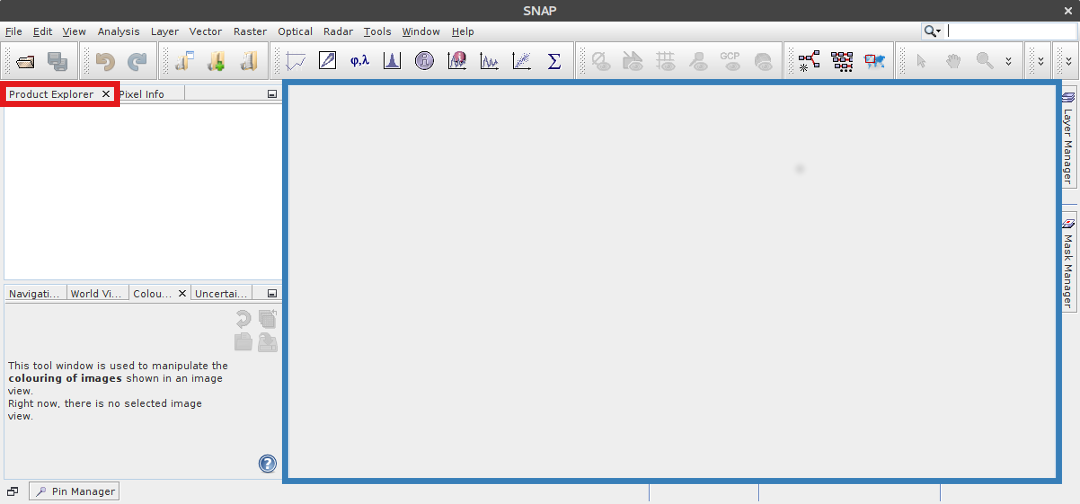
\includegraphics[scale=1.1]{fig:int.png}
    \caption{Interfáz gráfica del usuario. El árbol de capas y el área de visualización del programa.}
    \label{fig:int}
\end{figure}

\section{Apertura de imágenes}

En el menú principal, seleccione \emph{Open product...} y dentro de la carpeta \path{material/raster_data}, seleccione \path{S2A_MSIL2A_20170720.dim}.

Haga doble click sobre el nombre y se desplegará un árbol que incluye las siguientes opciones:
\dirtree{%
    .1 [1] S2\_MSIL2A\_20170702.
    .2 Metadaata.
    .2 Index Codings.
    .2 Vector Data.
    .2 Bands.
    .2 Masks.
}

De esta cobertura se destaca:

\begin{itemize}
    \item \emph{[1] S2\_MSIL2A\_20170702}: El número de elemento entre corchetes y el nombre de la imagen.
    \item \emph{Metadata}: Los metadatos asociados a la imagen y su historial de procesamiento.
    \item \emph{Index Codings}: Los valores de referencia de como interpretar dentro de la imagen y las máscaras distintos valores.
    \item \emph{Vector data}: Las capas vectoriales asociadas a la imagen.
    \item \emph{Bands}: Las bandas de la imagen y las operaciones de álgebra entre bandas. Haciendo doble click puede mostrarlas en el visualizador.
    \item \emph{Masks}: Las máscaras que sean incluidas en la imagen o las que crearán.
\end{itemize}

\section{Visualización}

Puede visualizar una de las bandas de la imagen haciendo doble click sobre ella. La banda se mostrará en escala de grises (Figura \ref{fig:mono})

\begin{figure}[h!]
    \centering
    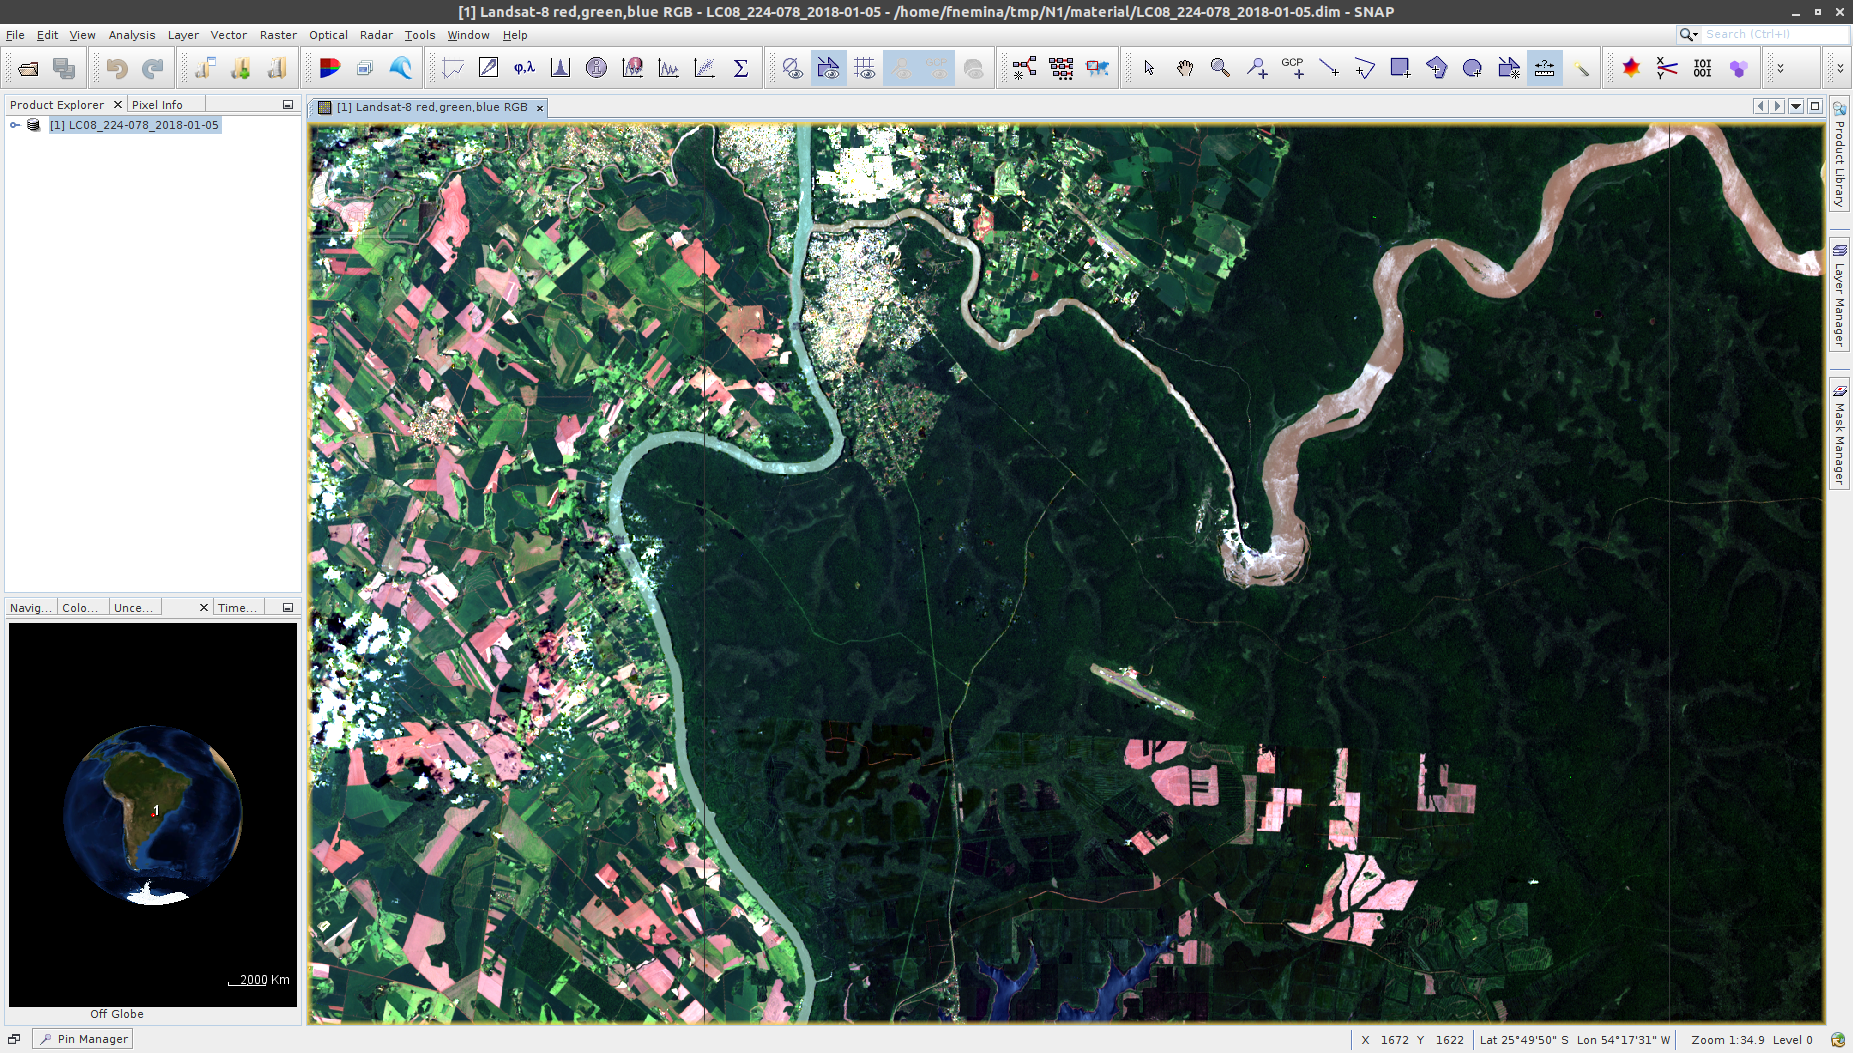
\includegraphics[scale=0.7]{fig:mono.png}
    \caption{Imagen monobanda desplegada en el visualizador.}
    \label{fig:mono}
\end{figure}

Es posible abrir varias bandas en simultaneo y cada una de ella se mostrará en una pestaña nueva.

Explore la imagen utilizando las herramientas de navegación y zoom (Figura \ref{fig:NAV})

\begin{figure}[h!]
    \centering
    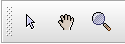
\includegraphics[scale=0.5]{fig:NAV.png}
    \caption{Herramientass de navegación. De izquierda a derecha: \emph{Selection tool}, para seleccionar objetos en la imagen, \emph{Panning tool}, para moverse dentro de la imagen, y \emph{Zooming tool}, para hacer zoom en la imagen.}
    \label{fig:NAV}
\end{figure}

En \emph{Product Explorer} haga click derecho sobre el nombre y seleccione \emph{Open RGB image windows.}. Se desplegará una nueva ventana (Figura \ref{fig:RGB}) que le permitirá elegir la combinación de bandas.

\begin{figure}[h!]
    \centering
    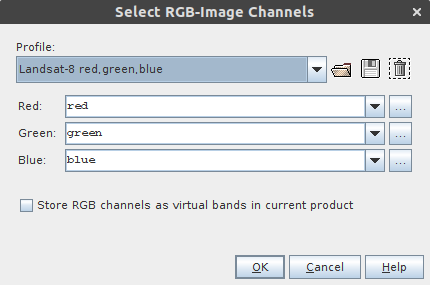
\includegraphics[scale=0.7]{fig:RGB.png}
    \caption{Ventana de combinación de bandas. Puede eligir una banda para cada canal del monitor ()\emph{Red, Green, Blue}) o puede optarpor una preseleccionada del menú \emph{Profile}}
    \label{fig:RGB}
\end{figure}

Por defecto elegirá la combinación que utiliza las bandas 4, 3 y 2 de Sentinel 2 y la desplegará haciendo click en OK (Figura \ref{fig:RVA}).

\begin{figure}[h!]
    \centering
    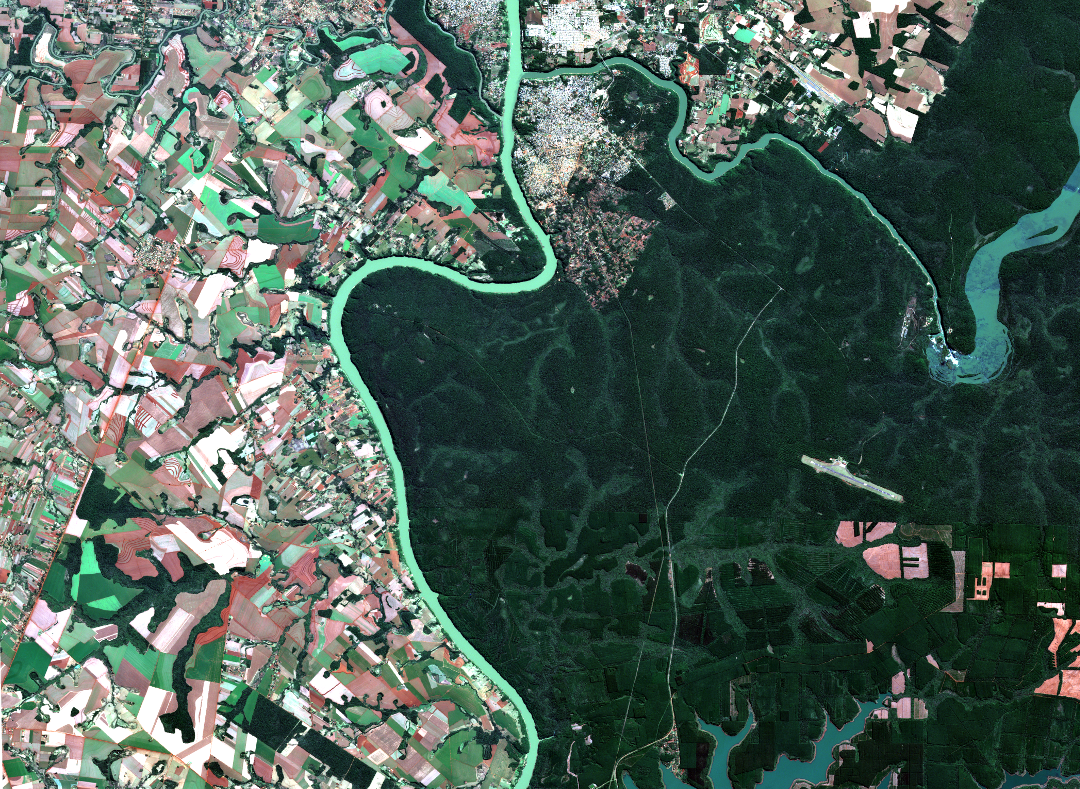
\includegraphics[scale=0.5]{fig:RVA.png}
    \caption{Imagen en combinación de colores de color real.}
    \label{fig:RVA}
\end{figure}


\section{Consulta de píxel}

Haciendo click en la pestaña píxel info es posible obtener la información sobre un píxel para todas las bandas que se encuentren abiertas.

Para utilizarla haga click en la pestaña \emph{píxel info} y posicionese sobre un píxel en la imagen (Figura \ref{fig:pixel}).

\begin{figure}[h!]
    \centering
    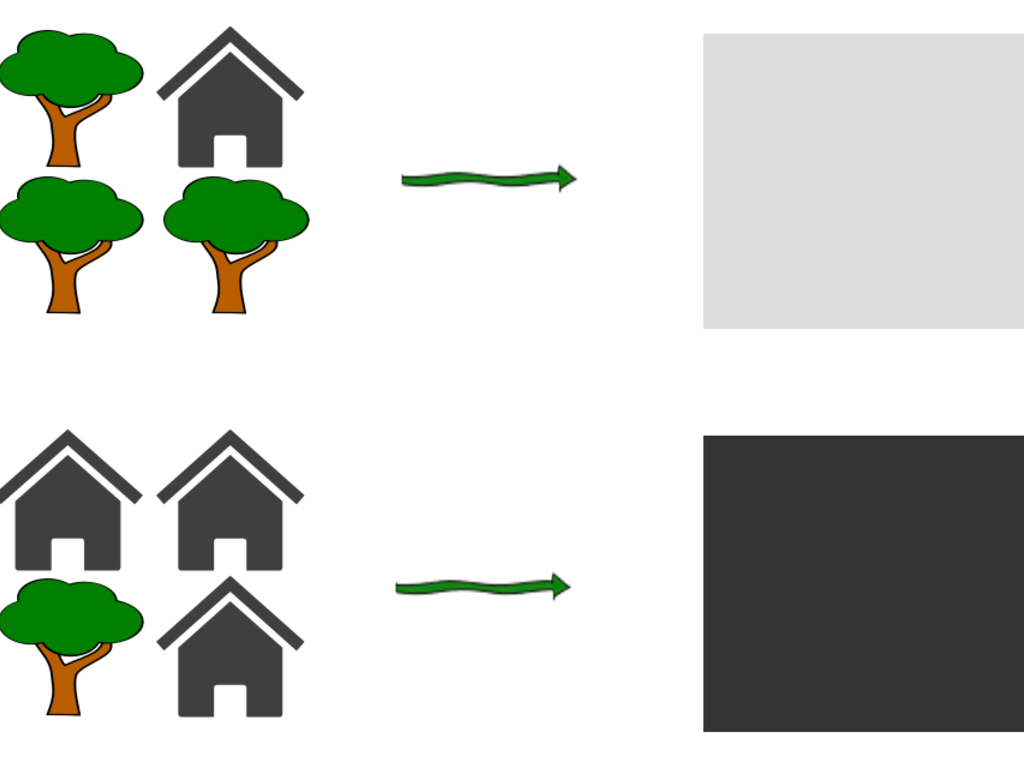
\includegraphics[width=0.3\textwidth]{fig:pixel.png}
    \caption{}
    \label{fig:pixel}
\end{figure}

Obsevará información que incluye el píxel en el que se encuentra, la latitud y longitud del píxel, las coordenadas dentro del mapa y el valor de la banda que se encuentre abierta.

\section{Actividad}

Abrá la imagen \path{S2A_MSIL2A_20170720} de la  carpeta \path{material/raster_data}. Abra la banda \path{Sigma0_VH}.

\begin{que}
    ¿A que coberturas dentro de la imagen pertenecen las regiones de la imagen con mayor nivel de brillo?
\end{que}

\begin{que}
    ¿Como es el valor de brillo para las zonas de cuerpos de agua?
\end{que}

\begin{que}
    ¿Cuales son las coordenadas aproximadas del aeropuerto que se encuentra en el centro de la imagen?
\end{que}
